\subsection{Projektphasen}
\label{sec:Projektphasen}

Nachdem im vorherigen Abschnitt die Organisation des Projektes erläutert wurde,
wird im Folgenden das Projekt in Phasen gegliedert. Die Phasen dienen 
dazu, das Projekt in einem geordneten Ablauf zu strukturieren und
Arbeitsschritte aufeinander aufbauend zu vergeben. "`Der Aufbau der
Projektphasen ist darauf ausgerichtet, systematisch und aufeinander aufbauend
zu 'lernen', um insgesamt eine optimale Entscheidungsprozedur zu
durchlaufen"'.\footnote{\citet{walter2006}}

Jede Projektphase stellt dabei eine in sich geschlossene Einheit dar, die aus
mehreren Arbeitspaketen und Meilensteinen bestehen kann. Arbeitspakete sind
dabei konkrete Arbeitsschritte, die von einer ausgewählten Person in einem
gewählten Zeitraum zu erfüllen sind. Jedes Arbeitspaket arbeitet auf die
Erfüllung des jeweils nächsten Meilensteines hin.

Meilensteine bilden wichtige, elementare "`Stationen"' in einem Projekt ab. Sie
strukturieren das Projekt durch zeitliches Festlegen von Teilzielen.
Darüber hinaus kann an den abgeschlossenen Meilensteinen
der Erfüllungsgrad des Projektzieles abgelesen werden.\footnote{\citet{schels2008}}

Jede Projektphase endet daher mit einem Meilenstein. Der Projektphasenplan mit
den jeweiligen abschließenden Meilensteinen ist in nachfolgender Abbildung
dargestellt:

\begin{figure}[htb] 
\centering
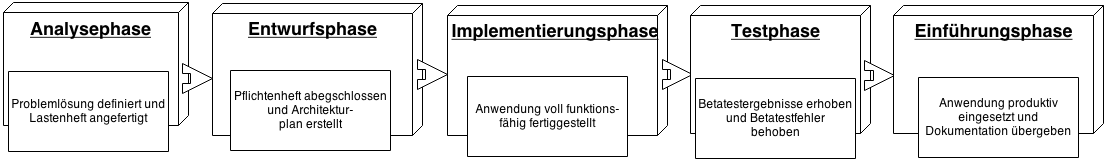
\includegraphics[width=1.0\textwidth]{Phasenplan.png}
\caption[Phasenplan des Projektes]{Phasenplan des Projektes\protect\footnotemark}
\label{fig:MockupFrontend}
\end{figure}
\footnotetext{eigene Darstellung}

\begin{description}

  \item[Die Analysephase] ist Ausgangspunkt der vorliegenden Projektarbeit. Sie setzt
  auf der aktuellen Ist-Situation an und in ihr werden Lösungsmöglichkeiten für
  das vorhandene Problem analysiert. Am Ende der Analysephase steht eine
  konzeptionelle Problemlösung. Das bedeutet konkret, aus der Analyse der
  vorliegenden Situation werden verschiedene Lösungsansätze entwickelt. Im
  Zuge der Analyse und Auswertung dieser Lösungsansätze wird ein Ansatz
  ausgewählt, der für die Lösung am geeignetsten ist. Die Analysephase ist in
  der vorliegenden Ausarbeitung im \verweis{Konzeptionierung} beschrieben.

  Die Ergebnisse der Analyse werden in einem Lastenheft\footnote{\citet{lastenheft2013}} formuliert.

  Die Analysephase wird mit dem Meilenstein "`Problemlösung definieren und
  Lastenheft angefertigt"' abgeschlossen.

  \item[Die Entwurfsphase] folgt im Anschluss auf die Analysephase.
  Ausgangspunkt der Entwurfsphase ist ein angefertigtes Lastenheft. Aufgrund der
  darin beschriebenen Anforderungen kann die Planung der Umsetzung
  begonnen werden. Die
  Entwurfsphase beinhaltet dabei Modelle und Entwürfe, 
  die konkret beschreiben, wie die
  Anforderungen des Lastenheftes umgesetzt werden. Das Ergebnis der Entwurfsphase ist ein erstelltes Pflichtenheft, das die konkretisierte Umsetzung des Problems
  beschreibt.

  Im vorliegenden Projekt wurden systematisch verschiedene Teilgebiete der
  entstehenden Lösung betrachtet und mit Modellen individuell konzipiert, um die
  Komplexität einer solchen Lösung in kleinere Teilbereiche zu unterteilen. Dabei
  wurden hauptsächlich die Bereiche Datenhaltung bzw. Datenbankdesign und
  Anwendungslogik voneinander getrennt betrachtet. Dieser getrennten Betrachtung
  ging dabei der Entwurf eines ersten Oberflächendesigns, ein sogenanntes
  Mockup, voraus. Mit diesem Mockup konnte ein erster Eindruck über Umfang und
  Komplexität gewonnen und zusätzlich Funktionalität und Benutzung
  verdeutlicht werden. Eine Abbildung dieses Mockups ist an Anhang ~\ref{sec:Mockup} zu sehen.

  Eine genauere Betrachtung der Entwurfsphase würde an dieser Stelle zu weit führen,
  kann aber in \citet{modelierungUndBetrieb2014} nachgelesen werden.
  Das angefertigte Pflichtenheft kann in \citet{pflichtenheft2013} nachgelesen werden.

  Die Entwurfsphase wurde mit dem Meilenstein "`Pflichtenheft abgeschlossen und
  Architekturplan erstellt"' abgeschlossen.

  \item[Die Implementierungsphase] folgt im Anschluss an die Entwurfsphase und
  baut auf einem abgeschlossenen Pflichtenheft auf. Diese Phase ist sowohl die
  zeitlich größte Phase als auch die Entscheidende, da in dieser Phase alle im
  Vorfeld geplanten Schritte und Modelle umgesetzt werden. In der Phase der
  Implementierung werden, aufbauend auf den vorher angefertigten Entwürfen, die
  theoretischen Modelle in ausführbaren Quellcode umgesetzt. In dieser Phase
  zeigt sich vor allem die Qualität der angefertigten Modelle, denn am
  schnellsten lässt sich Software entwickeln, wenn das dazugehörige Modell
  1:1 in Quellcode übertragen werden kann. Allerdings ist das, aufgrund der
  Schwierigkeit eine Software in seiner Komplexität in einem Modell zu erfassen,
  häufig schwer zu erreichen. Bei unerwartetem Abweichen vom Modell muss daher
  die Konzeption der Software erneut überdacht werden, um eventuellen logischen
  Fehlern vorzubeugen. Der Prozess dieser Implementierung kann in der
  Ausarbeitung Modellierung und Betrieb in Kapitel 5. (Umsetzung) nachgelesen werden.

  Die Implementierungsphase endet mit dem Meilenstein "`Anwendung voll
  funktionsfähig fertiggestellt"'.

  \item[Die Testphase] baut auf der fertigestellten und funktionierenden Software auf.
  Idealerweise wird der Test der Software von Personen durchgeführt, die nicht im Prozess der
  Softwareentwicklung beteiligt waren. Diese Personen haben eine
  unbeeinflusste Sicht auf die Software. Sie können so zum einen dessen
  intuitive Bedienung besser einschätzen und zum anderen benutzen sie die Software auch
  unvoreingenommen.Dies kann dazu führen, das sie Fehler in der Bedienung oder
  im Programm entdecken.Einen solchen Test, der von außenstehenden Personen
  durchgeführt wird, wird als Betatest bezeichnet. Diesem Betatest ist im
  Idealfall ein Alphatest der Entwickler vorausgegangen, in dem sie die entwickelten Anwendungsfälle (use cases) im fertigen Programm simulieren und dabei mögliche
  Fehler entdecken und ausbessern können. Der Alphatest wird in dieser Ausarbeitung nicht näher betrachtet,
  kann aber in \citet{modelierungUndBetrieb2014} nachgelesen werden.
  In der Betatestphase ist es besonders wichtig die  aufgetretenen Fehler
  und Kritiken zu erfassen und an die Entwickler weiterzugeben. Durch den
  Betatest können sogenannte "`Kinderkrankheiten"' früh erkannt und beseitigt
  werden. Das steigert die Qualität und erhöht vor allem die
  Benutzerzufriedenheit beim verwenden der Software. Die Betatestphase wird zudem im Folgenden
  zur Verifizierung von Projektzielen verwendet.\footnote{siehe \verweis{Zielkatalog}}

  Die Testphase wird mit dem Meilenstein "`Betatestergebnisse erhoben und
  Betatestfehler behoben"' abgeschlossen.

  \item[Die Einführungsphase] erfolgt nach erfolgreicher Fertigstellung der Software und Korrektur aller
  aufgetretenen Fehler. Die Software wird in dieser Phase dem Auftraggeber übergeben und produktiv eingesetzt.
  Zur Übergabe der Software gehört zudem eine Dokumentation der Funktionsweise, die im \verweis{Anwenderdokumentation} vorgestellt wird. Der Abschluss dieser Phase stellt damit den Abschluss des Projektes dar.

  Die Einführungsphase endet mit dem letzten Meilenstein "`Anwendung produktiv
  eingesetzt und Dokumentation übergeben"'.

\end{description}